\chapter{kmalloc}

The current implementation of the generic kernel memory allocator is largely
based on tutorial written by Marwan Burrelle\cite{Burelle:malloc}.

\section{Brief Description}

The current kernel memory allocator implementation is somewhat naive and
exploits some very simple techniques like the first fit algorithm for allocating
memory.

Idea of the first fit algorithm is to find a first large enough free block of
memory from an already allocated region of memory. This is done by traversing
the list of memory blocks and looking for sufficiently large block. This is
of course quite sub-optimal and better solutions has to be considered.

When a large enough block is found it's split in two halves so that the left
one corresponds to requested size and the right block is left free. All data
blocks are aligned to 4 byte access.

Fragmentation of memory blocks is tried to keep minimal by merging newly freed
block with neighboring blocks. This will at least keep all free blocks between
reserved blocks free but it doesn't help much if there is allocations of
different sizes that are freed independently. So current implementation is very
sub-optimal also in this area.

When kmalloc is out of (large enough) memory blocks it will expand its memory
usage by allocating a new region of memory from dynmem. Allocation is done in
1 MB blocks (naturally) and always rounded  to a next 1 MB.

\begin{figure}
\begin{verbatim}
    +-+------+-+---------+-+-------+
    |d|      |d|         |d|       |
    |e| DATA |e|  FREE   |e| DATA  |
    |s|      |s|         |s|       |
    |c|      |c|         |c|       |
    +-+------+-+---------+-+-------+
\end{verbatim}
\caption{Kmalloc blocks.}
\label{figure:kmalloc_blocks}
\end{figure}

Descriptors are used to store the size of the data block, reference counters and
pointers to neighbouring block descriptors.


\section{Suggestions for Further Development}

\subsection{Memory allocation algorithms}

Current implementation of kmalloc relies on first-fit algorithm and variable
sized blocks, that are processed as a linked list, which is obviously inefficient.

One possible improvement could be adding a second data structure that would
maintain information about free memory blocks that could be used to store the
most common object sizes. This data structure could be also used to implement
something like best-fit instead of first-fit and possibly with even smaller
time complexity than the current implementation.

\begin{eqnarray}
\mathrm{proposed\_size} &=& \mathrm{req\_size}
  + \frac{\mathrm{curr\_size}}{\mathrm{req\_size}} \mathrm{o\_fact}
  + \frac{\mathrm{curr\_size}}{o\_div}.
\end{eqnarray}

\begin{algorithm}
  \caption{krealloc over commit}
  \label{algo:realloc_oc}
  \begin{algorithmic}
      \If{$\mathrm{req\_size} > \mathrm{proposed\_size}$}
        \State $\mathrm{new\_size} \gets \mathrm{req\_size}$
      \Else
        \If{$\mathrm{limit}_{min} < 4 \frac{proposed\_size}{req\_size} < \mathrm{limit}_{max}$}
          \State $\mathrm{new\_size} \gets \mathrm{proposed\_size}$
        \Else
          \State $\mathrm{new\_size} \gets \mathrm{max(req\_size, curr\_size})$
        \EndIf
      \EndIf
  \end{algorithmic}
\end{algorithm}

This is however completely untested and intuitively derived method but it
seems to give a nice looking curves for hypothetical memory allocations as seen
in figure \ref{figure:realloc}.

\begin{figure}
  \center
  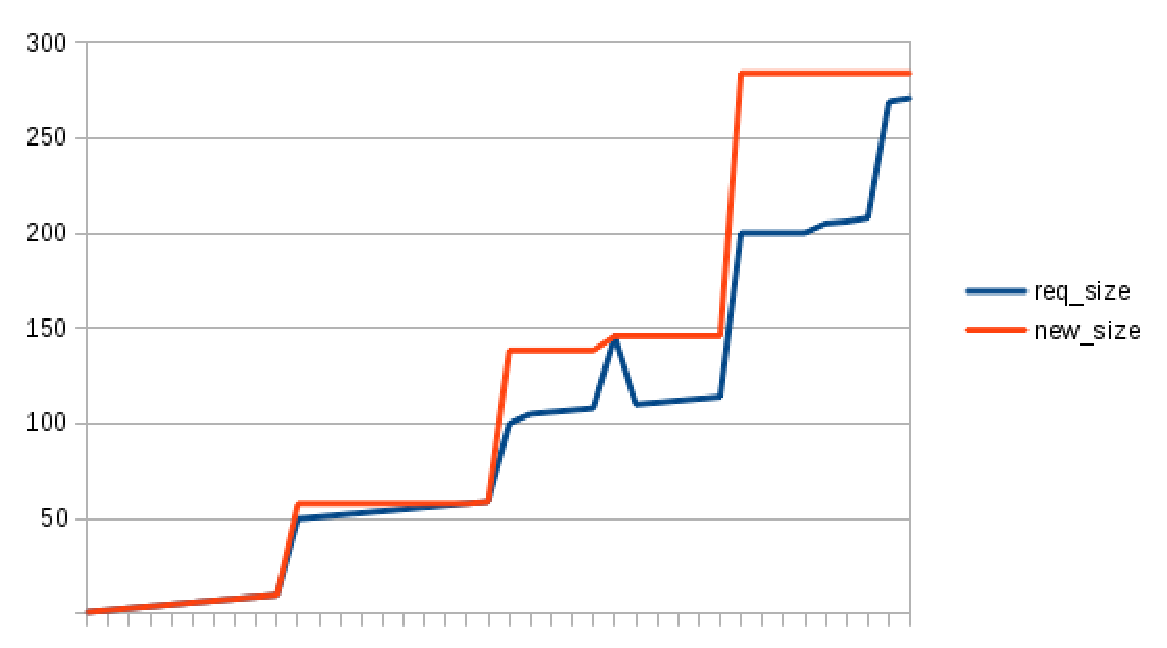
\includegraphics[width=10cm]{pics/realloc}
  \caption{New realloc method.}
  \label{figure:realloc}
\end{figure}
